%!TEX root = ../dissertation.tex
%\begin{savequote}[75mm]
%This is some random quote to start off the chapter.
%\qauthor{Firstname lastname}
%\end{savequote}

\chapter{Continuous adaptation for efficient machine communication}
\graphicspath{{./figures/nn_modeling/}}

%\section{Introduction}

Linguistic communication depends critically on shared knowledge about the meanings of words \cite{Lewis69_Convention}. 
However, the real-world demands of communication often require speakers and listeners to go \emph{beyond} dictionary meanings to understand one another \cite{clark_using_1996,HassonGhazanfar___Keysers12BrainToBrain,stolk2016conceptual}. 
The social world continually presents new communicative challenges, and agents must continually coordinate on new meanings to meet them. %adapted to the needs of the current interaction.
For example, consider a nurse visiting a bed-ridden patient in a cluttered home.
The first time they ask the nurse to retrieve a particular medication, the patient must painstakingly refer to unfamiliar pills, e.g.~``my vasoprex-tecnoblek meds for blood pressure, in a small bluish bottle, on the bookcase in my bathroom.''
After a week of care, however, they may just ask for their ``Vasotec.'' 

\begin{figure}[t]
\centering
\includegraphics[scale=.65]{frontfig.pdf}
\caption{Reference game task, listener architecture, and continual learning approach.}
\label{fig:refgame}
\end{figure}
This type of flexible language use poses a challenge for models of language in machine learning.
Approaches based on deep neural networks typically learn a monolithic meaning function during training, with fixed weights during use.
For an in-home robot to communicate as flexibly and efficiently with patients as a human nurse, it must be equipped with a continual learning mechanism. Such a mechanism would present two specific advantages for interaction and communication applications.
First, to the extent that current models have difficulty communicating in a new setting, an adaptive approach can quickly improve performance on the relevant subset of language.
Second, for human-robot contexts, an adaptive model enables speakers to communicate more efficiently as they build up common ground, remaining understandable while expending significantly fewer words as humans naturally do \cite{ClarkWilkesGibbs86_ReferringCollaborative}.

%For example, when a store sells a gadget they call a `slip joint plier,' a speaker of the language can assume it means the same thing as it meant the previous week, and the same thing meant by the store across town.
%For instance, a car repairman who needs to repeatedly ask her co-woker to pass the 'slip joint plier' may eventually adapt conventions and ask for the 'slip'. Humans are adept listeners and are able to understand adapted conventions, e.g., that both 'slip' and 'slip joint plier' refer to the same object.
%For example, many open problems in human-computer interaction require repeatedly referring to novel objects or locations or technical concepts, which may be quite costly and error-prone using existing conventions. \dots %\todo[inline]{refine examples}
In this chapter, we  introduce a general framework for transforming neural language models into \emph{adaptive} models that can be deployed in real-time interactions with other agents.
%\begin{quote}
Our key insight is that through continual interactions with the same partner in a shared context, a listener can adapt and more efficiently communicate with its partner (Fig.~\ref{fig:refgame}).
%\end{quote}
We are motivated by the hierarchical Bayesian approaches to task-specific adaptation from Chapter 2. 
We implement this theoretical approach at scale by integrating two core components: (i) a loss function combining speaker and listener information  
to understand descriptions of natural images in context, and (ii) a regularization scheme for fine-tuning the weights of this model based on previous interactions with a partner. %, and (iii) a data augmentation strategy to approximate the compositionality of utterances. 
We show that these components enable more effective communication with human partners over repeated interactions.

\section{Approach}
We begin by recasting communication as a multi-task problem for meta-learning. 
Each context and communicative partner can be regarded as a related but distinct task making its own demands on the agent's language model. 
To be effective across many such tasks, a communicative agent must both (1) have a good prior representation they can use to understand novel partners and contexts, and (2) have a mechanism to rapidly update this representation from a small number of interactions.
%The current work begins with a conventionally pre-trained initialization and focuses on developing the latter mechanism.

\subsection{Repeated reference game task}
As a benchmark for studying this problem, we introduce the \emph{repeated reference game} task (Fig. \ref{fig:refgame}), which has been widely used in cognitive science to study partner-specific adaptation in communication \cite{KraussWeinheimer64_ReferencePhrases,ClarkWilkesGibbs86_ReferringCollaborative,WilkesGibbsClark92_CoordinatingBeliefs}.
This task is a special case of the more general family of reference games, where a speaker agent is given a context of $N$ images (a target object $o$ among $N-1$ distractors) and must produce an utterance $u$ that allows their partner, a listener agent, to identify $o$ with high probability. 
In a \emph{repeated reference game}, each image in context appears as the target multiple times, allowing us to evaluate how communication about a particular image changes as the speaker and listener build up a shared history. 

\subsection{Continual adaptation with Hierarchical Bayes}
Before formalizing our algorithm as a generic update rule for neural networks, we describe the theoretical Bayesian foundations of our approach, reviewing material from previous chapters in the context of machine learning.
% \ndg{i generally think of this as the semantics, and a lexicon maps single words to meanings.... you could change or clarify, though i don't feel strongy}
Under a Bayesian approach, semantic representations can be viewed probabilistically: we represent some uncertainty over meanings.
%We define the lexicon as a function $\mathcal{L}: (w_n, o_m) \rightarrow \mathbb{R}$, assigning any word-object pair a real-valued meaning according to how well the word $w_n$ applies to the object $o_m$. 
%This is a continuous generalization of classic truth-conditional semantics. %\shortcite{graf_animal_2016}. 
%We view the lexicon not as a lookup table or a static logical form untouched after childhood, but as a dynamic, parameterized representation that is constantly being updated.
In a hierarchical Bayesian model, this uncertainty is structured over different partners and contexts.

At the highest level %of a hierarchical lexical representation 
is a \emph{task-general} variable $\Theta$ which parameterizes the agent's task-specific prior expectations $P(\theta_{i} | \Theta)$ where $\theta_i$ represents the semantics used by a novel partner $i$. 
Given observations $D_i$ from communicative interactions in that context, an agent can update their \emph{task-specific} model using Bayes rule:
\begin{equation}
	P(\theta_i | D_i, \Theta)  \propto P(D_i | \theta_i) P(\theta_i | \Theta)
	\label{eq:lexicon_update}
\end{equation}
The Bayesian formulation thus decomposes the problem of task-specific adaptation into two terms, a prior term $ P(\theta_i | \Theta)$ and a likelihood term $P(D_i | \theta_i)$.
The prior captures the idea that different language tasks share some task-general structure in common: in the absence of strong information about usage departing from this common structure, the agent ought to be regularized toward their task-general knowledge.
%This property is a form of the Bayes Occam's Razor.

The likelihood term accounts for needed deviations from general knowledge due to evidence from the current situation. 
The form of the likelihood depends on the task at hand.
For the referential communication task we consider here, $D_i = \{(u, o)_t\}$ contains paired observations of utterances $u$ and their objects of reference $o$ at time $t$.
These data can be viewed from the point of view of a speaker (generating $u$ given $o$) or a listener (choosing $o$ from a context of options, given $u$) \cite{SmithGoodmanFrank13_RecursivePragmaticReasoningNIPS,HawkinsFrankGoodman17_ConventionFormation}; these yield different likelihoods that update the semantics in complementary ways.
The generative model of a \emph{speaker} uses the task-specific semantics $\theta_i$ to sample utterances $u$ proportional to how well they apply to $o$:
\begin{equation}
	P_S(u | o, \theta_i) \propto \exp f_{\theta_i}(u, o)
	\label{eq:speaker}
\end{equation}
A \emph{listener} can be modeled as inverting this speaker model to evaluate how well an utterance $u$ describes each object $o$ \emph{relative to the others} in a context $\mathcal{C}$ of objects by normalizing \cite{FrankGoodman12_PragmaticReasoningLanguageGames,VedantamEtAl17_ContextAwareCaptions,cohn2018pragmatically,MonroeEtAl17_ColorsInContext}:
\begin{equation}
 P_L(o | u, \mathcal{C}, \theta_i) \propto 
   P_S(u | o, \theta_i )P(o) % \frac{}
%          {\sum_{o_k \in \mathcal{C}} \exp(P(u | o_k, \mathcal{L}_i)) }	
	\label{eq:listener}
\end{equation}
Because these views of the data from past interactions $D_{i}$ provide complementary statistical information about the task-specific semantics $\theta_i$, we will combine them in our loss.
%Thus, in order to create adaptive listeners, we need to first model how adaptive speakers update $P(\mathcal{L}_i | D_i, \Theta)$. %/todo[inline]{explain why we need to model adaptive speakers for adaptive listeners}

\subsection{Continual adaptation for neural language models}


While the $N \times M$ word-object matrix used as the semantics in Chapter 2 cannot straightforwardly generalize to unseen words and objects. 
It also quickly becomes intractable as the vocabulary and object set grows, making it untenable for modeling arbitrary natural language.
Here we will instead take $\Theta$ to be an initialization for the weights of an image-captioning neural network (see Fig. \ref{fig:arch}A).
%Because the Rational Speech Act framework used throughout this proposal as a linking function %for discriminative production and interpretaion in context 
%has successfully been implemented on top of such CNN-RNN networks in previous work \shortcite{vedantam_context-aware_2017}, the key implementation bottleneck is not the parameterization or the linking function, but the inference algorithm.
 %We omit mathematical details here due to the conceptual nature of the article, but a full account of the non-hierarchical version of this model can be found in \citeA{hawkins_convention-formation_2017}.

While it is theoretically possible to place priors on all neural network parameters and attempt to jointly approximate posteriors \shortcite{joshi_personalizing_2017}, current techniques for inference in Bayesian neural networks rely on optimization of noisy gradients of variational objectives and tend not to work well. 
Instead, because maintaining full hyper-priors is costly and challenging for inference, we will assume agents only represent an \emph{empirical Bayes} point estimate of $\Theta$ \cite{gelman_bayesian_2014}.
Additionally, we exploit a deep theoretical connection between the hierarchical Bayesian framework presented in the previous section and recent deep learning approaches to multi-task learning \cite{nagabandi_deep_2018,grant_recasting_2018,jerfel_online_2018}. 
Given a task-general initialization, regularized gradient descent on a particular task is equivalent to conditioning on new data under a Bayesian prior.
We exploit this connection to propose an online continual learning scheme for a neural listener model that can adapt to a human speaker in a challenging referential communication task.

Concretely, we consider an image-captioning network that combines a convolutional visual encoder (ResNet-152) with an LSTM decoder \cite{vinyals_show_2015}.
The LSTM takes a 300-dimensional embedding as input for each word in an utterance and then uses a softmax layer to linearly project back to a distribution over the vocabulary size.
An adapter replacing the final fully connected layer of the encoder was jointly pre-trained with the decoder on the COCO training captions and then frozen as our task-general initialization $\Theta$.
 % by the weights of an encoder network and a decoder network, $\{\Theta_E, \Theta_D\}$. 
For each utterance-object data point observed in the current task, we take a small number of gradient steps fine-tuning the decoder's weights to better account for the speaker's usage (see Algorithm \ref{alg:listener_update}).
%An adapting listener evaluates how well an utterance describes a context of images. We use our model of an adapting speaker to assess how well an utterance describes an image, $P(u_n | o_m, \mathcal{L}_i)$ %TODO not clear why we need an adapting speaker?
%After generating likelihoods for all images in a context, we normalize over our likelihoods to create a probability distribution over images, \eref{eq:listener}. 
We consider several loss terms and techniques to do so.

\begin{algorithm}[tb] %TODDO make this compatible with listener update!
	\caption{: Update step for adaptive language model}
    \label{alg:listener_update}
\begin{algorithmic}
    \STATE {\textbf{Input}: $\theta_t$: weights at time $t$}
    \STATE {\textbf{Output}: $\theta_{t+1}$: updated weights}
    \STATE {\textbf{Data}: ($u_t, o_t$): observed utterance and object at time $t$}
    \FOR{step}
        \STATE sample augmented batch of sub-utterances $\textbf{u} \sim \mathcal{P}(u)$
        \STATE update $\theta_t \leftarrow \theta_t + \beta\nabla[P(\bold{u} | o) + P(o | \bold{u})  + \text{reg}(o,u)]$
   \ENDFOR
\end{algorithmic}
\end{algorithm}

\paragraph{Speaker and listener likelihood.} 
The primary signal available for adaptation is the (log-) probability of the new data under speaker and listener likelihoods given in Eqns. \ref{eq:speaker}-\ref{eq:listener}.
Our speaker likelihood serves to make the observed utterance more likely for the target in \emph{isolation}, while our listener likelihood makes it more likely \emph{relative} to other objects in context. %, thus learning to differentiate between objects. 
The speaker and listener likelihoods can be computed directly from the neural captioning model, where each word is distributed according to a softmax over the LSTM output given the sentence so far.
%
%The \emph{speaker likelihood} directly approximates Eq. \ref{eq:speaker} using a neural captioning model %using teacher forcing \cite{williams1989learning}.%, summing the log probability of each word in the observed utterance $u$ conditioned on previous words. 
%by summing the log probabilities of each word $w_i\in u$ under the soft-max output of the decoder:
%$$P(u | o) =  -\sum\log p(w_i | o, w_{i-1})$$ %-\log p(u | o) =
%This is the standard log likelihood loss used to train captioning models.
%%Following the gradient through this loss term adjusts weights to make the observed caption more likely for the target of reference.
%%We take inspiration from these methods of association and introduce novel \emph{listener loss and regularization functions} in addition to considering commonly used loss and regularization functions, which we call the \emph{speaker loss and regularization functions}. 
%%Given an image, we take the cross-entropy loss between a distribution of utterances produced by our adapting speaker model $u$ and an utterance from our dictionary $u_i^* \in D^*$: 
%%\begin{equation}
%%	\text{loss}_S(u, \text{class}(u_i^*)) = -log\bigg(\frac{\exp(u[\text{class}(u_i^*)])}{\sum_j\exp(u[j])}\bigg)	
%%	\label{eq:speaker_loss}
%%\end{equation}
%The same model can also be used to compute the \emph{listener likelihood} %of selecting the target object $o$ 
%by computing the probability $P(u|o_i)$ for each object as above and then renormalizing to obtain a distribution over the context (Eq. \ref{eq:listener}).
%%$$\text{loss}_L = -\log(p(u | o)) - \log(\sum
%%Given an utterance $u$, the conditional probability distribution over the context $u \in \mathbb{R}^M$ %TODO omg fix this notation for distributions!
%% is given by $P(o_m | u_i^*, \mathcal{L}_i),\  m \in \ldots M$. 
%%For a target image $o_t$ and its respective utterance $u_i^*$, we take the cross-entropy loss between the distribution over the context and the target image: 
%%\begin{equation}
%%	\text{loss}_L(u, \text{index}(o_t)) = -log\bigg(\frac{\exp(u[\text{index}(o_t)])}{\sum_j\exp(u[j])}\bigg)	
%%	\label{eq:listener_loss}
%%\end{equation}

\paragraph{Regularization.} 
We introduce three kinds of regularization terms to approximate the Bayesian prior on task-specific learning.
First, rather than directly regularizing weights, a \emph{speaker KL regularization} term minimizes the divergence between the captioning model's output probabilities before and after fine-tuning \cite{yu2013kl, galashov_information_2018}. %.
%This approach has been popular in adaptive speech processing \cite{yu2013kl} and reinforcement learning \cite{galashov_information_2018}.% but has not to our knowledge been used for interpretation.
Since the support for our distribution of captions are infinite, we approximate the divergence incrementally by expanding from the maximum a posteriori (MAP) word at each step according to $P$, where $P$ represents the model at initialization and $Q_t$ represents the model at time $t$. 
This loss is then averaged across random images from the full domain $\mathcal{O}$, not just those in context:
\begin{equation}
	\sum_{o\sim\mathcal{O}}
	 			 \sum_i 
				 D_{\mathrm{KL}}
				 \left(
				 P(w_i |o, w^{\mathrm{MAP}}_{i-1})
				 ||
				 Q_t(w_i|o, w^{\mathrm{MAP}}_{i-1})
				 \right)
\label{eq:speaker_reg}
\end{equation}
Second, we derive a \emph{listener KL regularization} term which compares the initial listener distribution over objects in context $o \in \mathcal{C}$ with the fine-tuned model's distribution: $D_{\mathrm{KL}}\left(P(o | u)||Q_t(o | u)\right).$
%In principle, this term restrains the model from overfitting to particular contexts.
%\begin{equation*}
%\begin{split}
%\end{split}
%\label{eq:listener_reg}
%\end{equation*}
%\paragraph{Task-specific history rehearsal} 
The third form of regularization we consider is \emph{local rehearsal}.
We evaluate our listener likelihood over prior observations $(u,o) \in D_i$ to prevent overfitting to the most recent observation.
To capture how the likelihood overwhelms the prior with increasing data in Bayesian updating, we anneal the listener regularization and rehearsal over the course of interaction while reverse-annealing the listener likelihood.

\paragraph{Data augmentation.} A final component of our algorithm is the introduction of a data augmentation step on the new utterance $u$.
Ideally, an adaptive agent should learn that sub-components of the observed utterance are compositionally responsible for this meaning.
%This fine-tuning approach strengthens the association between sub-utterances of an utterance and its respective image. 
We thus derive a small training dataset $D(u)$ from $u$; 
% For each utterance $u_i^0 \in U^0_i$, we can parse it using a syntactic parser (Allen NLP's Constituency Parser) to create $\hat{U_i^t}$. 
for simplicity, we take the (ordered) powerset $D(u) = \mathcal{P}(u)$ of all sub-utterances.\footnote{Grammatical acceptability could in principle be taken into account using alternative sets derived from a syntactic parse.}
%For each reduced utterance $\hat{u}_i^t$, we then feed it into a function that evaluates how uniquely it describes a particular image. 
%We choose the reduced utterance with the score that is highest for the target image (and lower for the rest of the images). 
%We then update weights in the neural network and update $u^{t+1}_i \leftarrow \hat{u}^t_0$. 
%With the updated utterance $u^{t+1}_i$ we then repeat steps 3-5. 
%We are able to create an adaptive speaker that is able to both model and produce shorter, adapted utterances over time. 

 %TODO fill listener reg in 

\section{Evaluations}

%We constructed three kinds of contexts from images in the COCO validation set to obtain varying degrees of communicative difficulty. 
To evaluate our model, we implemented a repeated reference game using images from the validation set of COCO \cite{lin2014microsoft} as the targets of reference.
To construct challenging contexts $\mathcal{C}$, we used our pre-trained visual encoder to find sets of highly similar images. 
%For \emph{far} contexts, we sampled images randomly from different COCO categories; in \emph{close} contexts, we sampled images from the same category (e.g. `giraffes`); and for \emph{challenge} contexts, 
We extracted feature vectors for each image, partitioned the images into 100 groups using a $k$-means algorithm, sampled one image from each cluster, and took its 3 nearest neighbors in feature space, yielding 100 unique contexts of 4 images each\footnote{Using pre-trained VGG as the encoder gave qualitatively similar contexts.}.

\subsection{Human baselines}


\begin{figure*}[t]
\centering
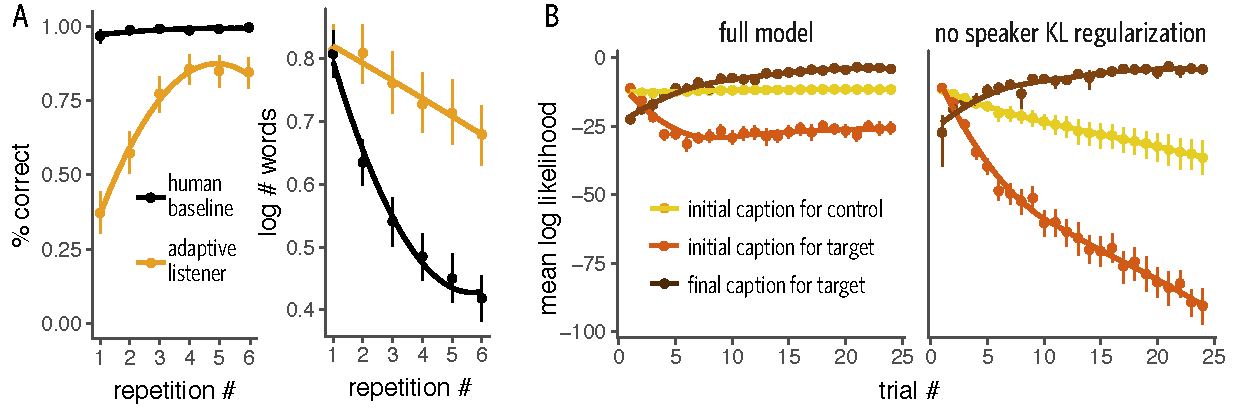
\includegraphics[scale=0.7]{combinedResults.pdf}
%\vspace{-2em}
\caption{(A) Human speakers grow more efficient and accurate as our model adapts. Curves show regression fits. (B) Speaker KL regularization prevents catastrophic forgetting. Error bars and ribbons are bootstrapped 95\% CIs.}
\vspace{-1em}
\label{fig:results}
\end{figure*}

We first investigated the baseline performance of human speakers and listeners. % in our repeated reference game task.
We recruited 113 participants from Amazon Mechanical Turk and automatically paired them into an interactive environment with a chatbox.
For each of these 56 pairs, we sampled a context and constructed a sequence of 24 trials structured into 6 repetition blocks, where each of the 4 images appeared as the target once per block. 
We prevented the same target appearing twice in a row and scrambled the order of the images on each player's screen on each trial. 
%To avoid referring expressions like ``same as last round'' or ``the one on the left,'' w
%Players were given a small bonus for each correct response.

We found that pairs of humans were remarkably accurate at this task, with performance near ceiling on every round.
At the same time, they grew increasingly efficient in their communication: the utterance length decreased from an average of 7 words per image on the first repetition to only 3 words on the last.
%While we observed variability across pairs% in both their overall utterance length and the extent of their reduction
A mixed-effects regression with random slopes and intercepts accounting for variability at the pair- and context-level found a significant decrease in utterance length across repetitions, $t=-5.8, p < 0.001$ (Fig. \ref{fig:results}A).
%, with a significant quadratic component, $t = 8.3, p < 0.001$ indicating that reduction gradually asymptotes 

\subsection{Model evaluation with human partner}

Next, we evaluated how our adaptive listener performed in \emph{real-time interaction} with human speakers. 
We recruited 45 additional participants from Amazon Mechanical Turk who were told they would be paired with an artificial agent learning how they talk.
This task was identical to the one performed by humans, except participants were only allowed to enter a single message through the chatbox on each trial. 
This message was then sent to a GPU where the model weights from the previous trial were loaded, used to generate a response, and updated in real-time for the next round.
The approximate latency for the model to respond was 6-8 seconds.

%\todo[inline]{Not sure how to cite the pytorch tutorial by Yunjey Choi that we took our pre-trained network from...}
We used a batch size of 8, learning rate of 0.0005, and took 8 gradient steps after each trial. 
For our loss objective, we used a linear combination of the speaker likelihood loss, listener likelihood loss, and all three regularization terms.
We found that a listener based on a pre-trained neural captioning model---the initialization for our adapting model---performs much less accurately than humans due to the challenging nature of the reference task. 
Yet our model rapidly improves in accuracy as it coordinates on appropriate meanings with human speakers.
Similarly, while speakers did not simplify their utterances to the same extent as they did with other humans, perhaps due to early feedback about errors, they nonetheless became significantly more efficient over time, $b = -19, t = -5$ (see Fig. \ref{fig:results}A).
%Before considering the full reference game context, we show that our fine-tuning scheme leads to systematic utterance reduction with a single image in isolation.
%We took K images from the coco dataset, and for each image, we used a pre-trained image-captioning model \cite{XXX} to sample an initial utterance (average length XX).
\section{Analysis}

%Having shown that the full loss allows our listener agent to achieve more accurate and efficient communication with a human partner
We proceed to a series of lesion analyses that analyze the role played by each component of our approach.
%We now proceed to a series of lesion analyses that allow us to understand the role played by each component of our approach.

%\begin{figure}
%\centering
%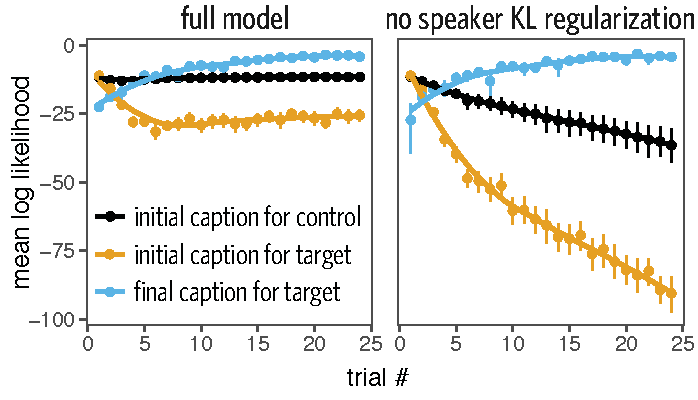
\includegraphics[scale=0.7]{../figures/catForgettingResults.pdf}
%\vspace{-2em}
%\caption{Lesioning the speaker KL regularization term leads to catastrophic forgetting. Error bars are bootstrapped 95\% CIs.}
%\vspace{-1em}
%\label{fig:forgetting}
%\end{figure}
%
%
%\begin{figure}[t]
%\centering
%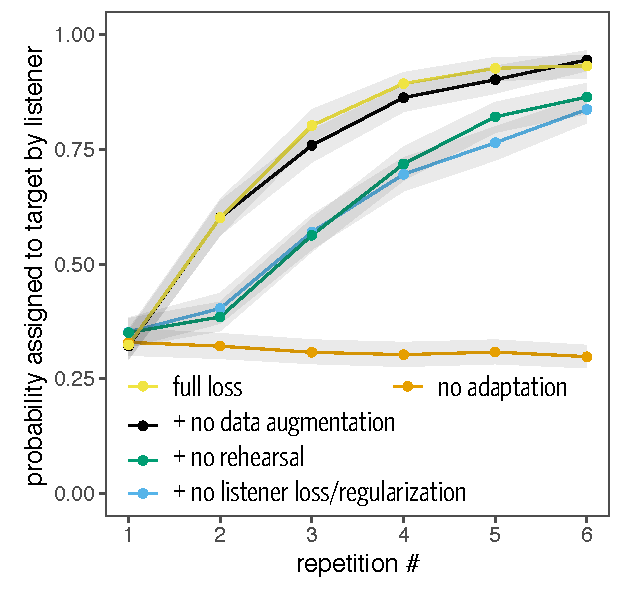
\includegraphics[scale=0.5]{../figures/lossComparisonResults.pdf}
%\vspace{-1.5em}
%\caption{The effect of lesions on simulated listener performance. Error ribbons are bootstrapped 95\% CIs.}
%\vspace{-1em}
%\label{fig:losses}
%\end{figure}

\begin{figure*}[t]
\centering
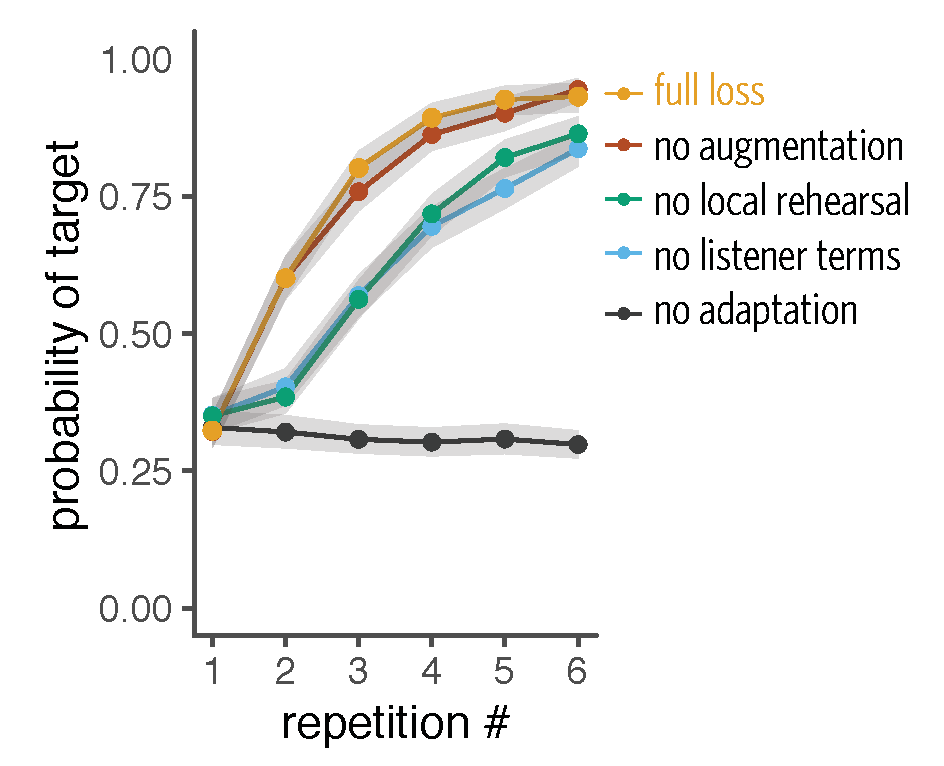
\includegraphics[scale=0.5]{lossLesions.pdf}
\caption{Lesions reveal the contributions of each loss term. Error bars and ribbons are bootstrapped 95\% CIs.}
\label{fig:results}
\end{figure*}

\subsection{Preventing catastrophic forgetting}
%First, we examine the role played by our regularization terms.
Fine-tuning repeatedly on a small number of data points presents a clear risk of catastrophic forgetting \cite{robins_catastrophic_1995}, losing our ability to produce utterances for other images. % it had previously been trained on. 
Our speaker KL regularization (Eqn.~\ref{eq:speaker_reg}) was intended to play the same role as a Bayesian prior, preventing catastrophic forgetting by tethering task-specific behavior to the task-general model.
To test the effectiveness of this term, we examined the likelihood of different captions before and after adaptation to the human baseline utterances. 
First, we sampled a random set of images from COCO that were not used in our experiment as \emph{control} images, and used the initialized state of the LSTM to greedily generate a caption for each.
We also generated initial captions for the \emph{target} objects in context. % used in our evalutions.
We recorded the likelihood of all of these sampled captions under the model at the beginning and at each step of adaptation until the final round. 
Finally, we greedily generated an utterance for each target at the end and retrospectively evaluated its likelihood at earlier states.
These likelihood curves are shown with and without speaker KL regularization in Fig.~\ref{fig:results}B.
The final caption becomes more likely in both cases; without the KL term, the initial captions for both targets and unrelated controls are (catastrophically) lost.
 
\subsection{Lesioning loss terms}

%Having established that the speaker KL regularization is key for reducing forgetting, 
We next simulated our adaptive listener's performance hearing utterances from the human baseline under lesioned losses (Fig. \ref{fig:results}C). 
We found that rehearsal on previous rounds had the largest qualitative benefit, allowing for faster adaptation on early rounds, while data augmentation and the non-rehearsal listener terms provided small boosts later in the game.
Compared to a non-adapting baseline, however, even a simple loss only containing the speaker likelihood and speaker KL regularization performed better over time---successfully adapting to human language use.

\section{Discussion}

Human language use is flexible, continuously adapting to the needs of the current situation. 
In this paper, we introduced a challenging repeated reference game benchmark for artificial agents, which requires such adaptability to succeed. 
We proposed a continual learning approach that forms context-specific conventions by adapting general-purpose semantic knowledge.
Even when models based on general-purpose knowledge perform poorly, our approach allows human speakers working with adapted variants of such models to become more accurate and more efficient over time.
%More broadly, recognizing the tasks language is put to is a first step toward a meta-learning approach to learn better initializations.

% Good to have the following format:
% Summary.
% Limitations.
% Future Work.